\chapter{Tecniche di Rappresentazione di Grafi}\label{app:csr}

    In questo capitolo sono descritte due delle principali tecniche utilizzate per rappresentare i grafi: la rappresentazione a matrice di adiacenza e la rappresentazione \textit{Compressed Sparse Row}.

    \section{Rappresentazione dei Grafi con Matrici di Adiacenza}
        Una matrice di adiacenza è una rappresentazione comunemente utilizzata per descrivere un grafo $G = (V, E)$, dove $V$ è l'insieme dei vertici e $E$ è l'insieme degli archi (o collegamenti) tra i vertici. Questa tecnica rappresenta il grafo come una matrice quadrata di dimensioni $|V| \times |V|$, con le seguenti caratteristiche:

        \begin{itemize}
            \item ogni riga e colonna della matrice corrisponde a un vertice del grafo;
            \item il valore in posizione $(i, j)$ della matrice indica se esiste un arco tra il vertice $i$ e il vertice $j$;
            \item per grafi non pesati, l'elemento $A[i][j]$ è uguale a 1 se esiste un arco tra $i$ e $j$, altrimenti è uguale a 0;
            \item per grafi pesati, l'elemento $A[i][j]$ contiene il peso dell'arco tra $i$ e $j$ (se esiste), mentre un valore predefinito, come $\infty$ o 0, è usato per indicare l'assenza di un arco;
            \item per grafi non orientati, la matrice di adiacenza è simmetrica rispetto alla diagonale principale, poiché un arco tra $i$ e $j$ implica anche un arco tra $j$ e $i$.
        \end{itemize}
    
        Questo tipo di rappresentazione è particolarmente utile per grafi densi, dove la maggior parte dei vertici sono connessi tra loro, poiché richiede $O(|V|^2)$ spazio di memoria.
    
        La matrice di adiacenza offre un modo semplice e diretto per eseguire operazioni come la verifica dell'esistenza di un arco tra due vertici, con una complessità $O(1)$. Tuttavia, può diventare inefficiente in termini di spazio di memoria per grafi molto sparsi, dove il numero di archi è significativamente inferiore a $|V|^2$. In questi casi, altre tecniche di rappresentazione, come le liste di adiacenza o il formato CSR per matrici sparse, possono essere più appropriate.


    \section{Compressed Sparse Row}
    
        Una matrice sparsa memorizzata in formato CSR (\textit{Compressed Sparse Row}) è una rappresentazione compatta che si basa sul memorizzare solo gli elementi non nulli della matrice. Questa tecnica è particolarmente utile per matrici sparse di grandi dimensioni, dove la maggior parte degli elementi è zero, riducendo drasticamente lo spazio di memoria richiesto rispetto alla memorizzazione di una matrice completa. Nel formato CSR, la matrice è rappresentata dai seguenti parametri:
    
        \begin{itemize}
            \item il numero di righe nella matrice;
            \item il numero di colonne nella matrice;
            \item il numero di elementi non nulli (\textit{nnz}) nella matrice;
            \item i puntatori all'array degli offset delle righe, di lunghezza pari al numero di righe $+ 1$, che rappresentano la posizione iniziale di ciascuna riga negli array delle colonne e dei valori;
            \item i puntatori all'array degli indici delle colonne, di lunghezza \textit{nnz}, che contiene gli indici delle colonne degli elementi corrispondenti nell'array dei valori;
            \item i puntatori all'array dei valori, di lunghezza \textit{nnz}, che contiene tutti i valori non nulli della matrice, ordinati in base alle righe.
        \end{itemize}

        La rappresentazione CSR permette di effettuare operazioni come il prodotto matrice-vettore in modo più efficiente, poiché si evita di processare esplicitamente gli elementi nulli. Inoltre, poiché gli elementi non nulli sono memorizzati in forma compatta, si riduce notevolmente il consumo di memoria \cite{NvidiaWebsite}.
        
        La Figura \ref{fig:graph-example} mostra un grafo orientato con 5 vertici mentre la Figura \ref{fig:csr-example} mostra come la rete si possa rappresentare secondo le due tecniche appena viste.
        
        \begin{figure}[h]
            \centering
            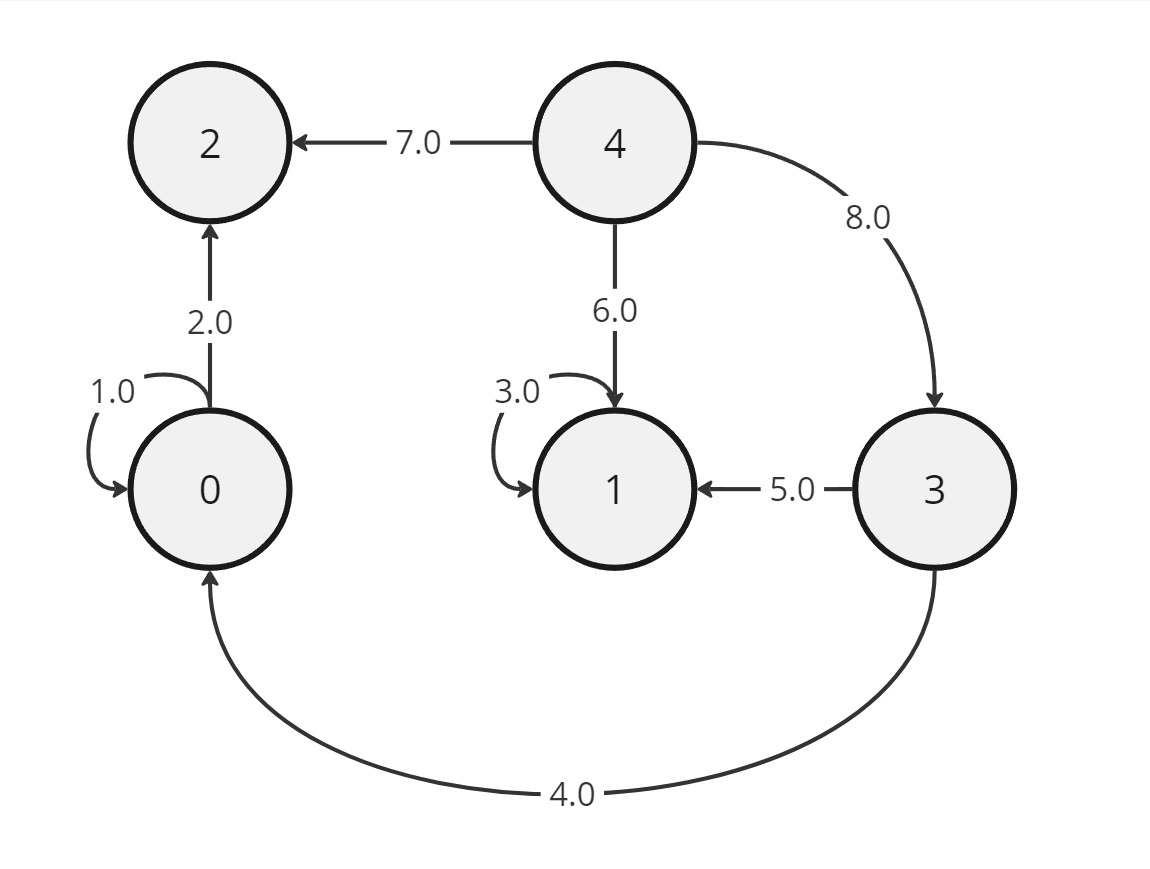
\includegraphics[width=0.5\linewidth]{images/graph.jpg}
            \caption{Esempio di grafo diretto pesato}
            \label{fig:graph-example}
        \end{figure}

        \begin{figure}[h]
            \centering
            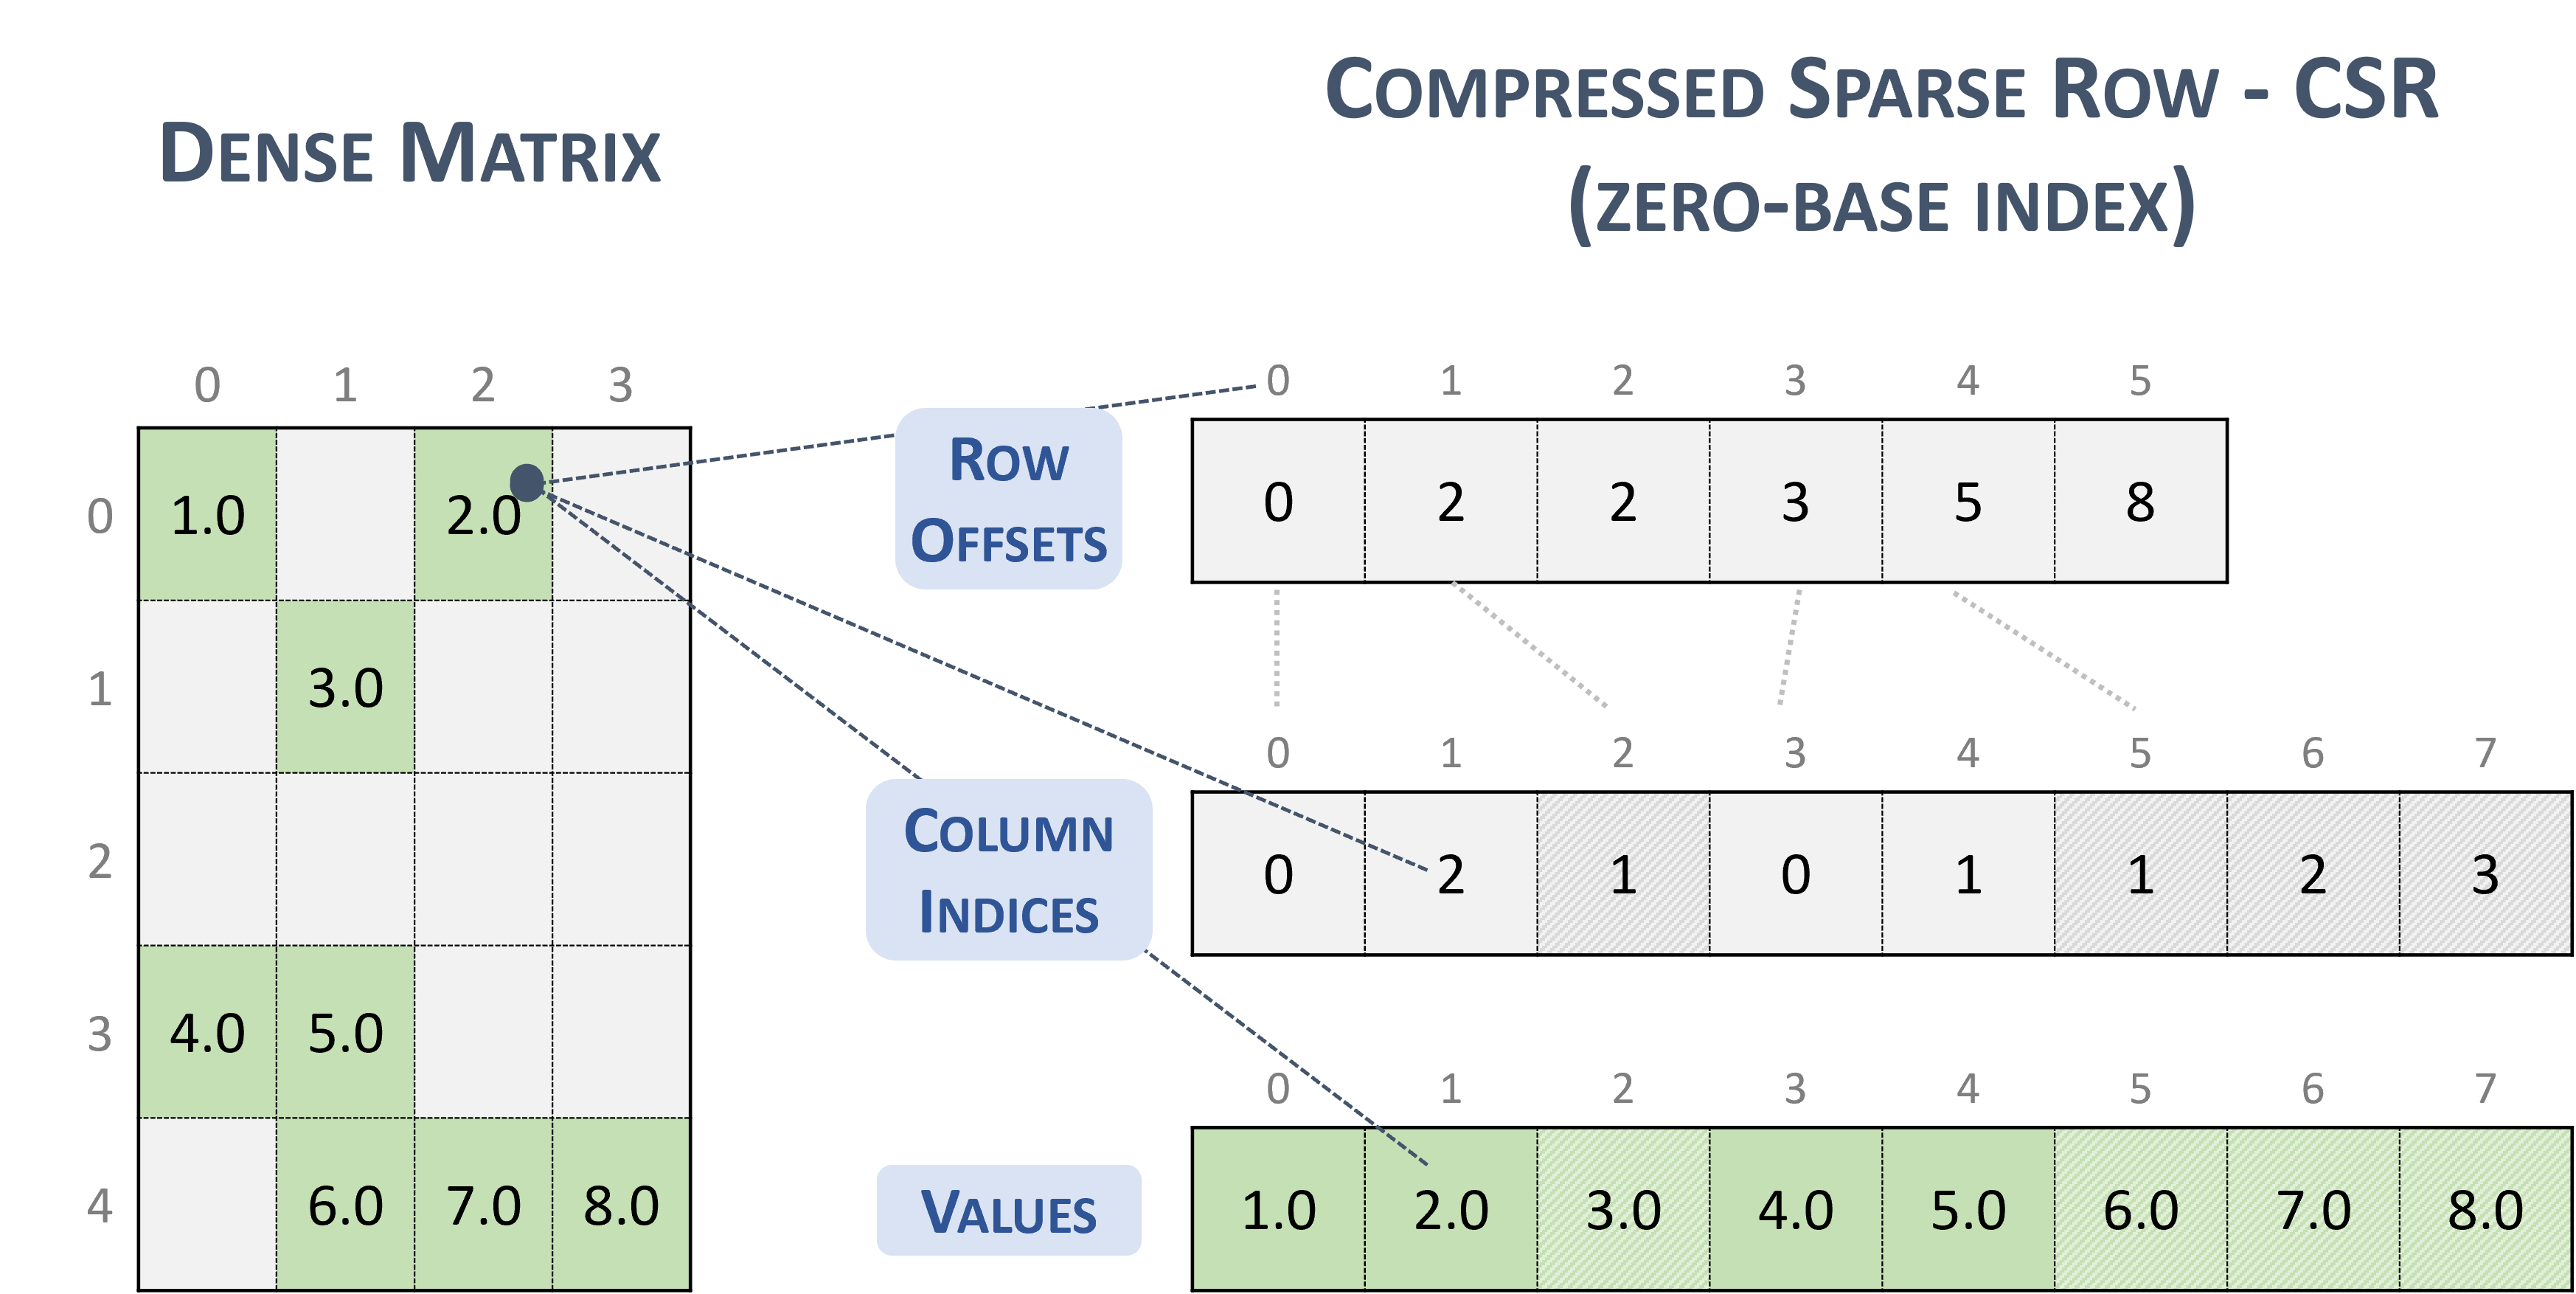
\includegraphics[width=0.9\linewidth]{images/csr-example.png}
            \caption{Matrice di adiacenza vs CSR}
            \label{fig:csr-example}
        \end{figure}
